\section{uTCA.4 Overview}

MicroTCA (uTCA) is Sinara's preferred form-factor for hardware with
high-speed data converters requiring deterministic phase control, such
as the \href{Sayma}{\emph{Sayma}} 2.4 GSPS smart arbitrary waveform
generator (SAWG).

uTCA is a modular, open standard originally developed by the
telecommunications industry. It allows a single rack master -- the Micro
TCA Carrier Hub (MCH) -- to control multiple slave boards, known as
Advanced Mezzanine Cards (AMCs) via a high-speed digital backplane. uTCA
chassis and backplanes are available commercially of the shelf (COTS).

We make use one of the most recent extension to the uTCA standard, uTCA.4.
Originating in the high-energy and particle physics (HEPP) community,
uTCA.4 introduces rear-transition modules (RTMs) along with a second
backplane for low-noise RF signals (RFBP). Each RTM connects to an AMC
(one RTM per AMC). Typically, the AMCs hold FPGAs and other high-speed
digital hardware, communicating with the MCH via gigabit serial links
over the AMC backplane. The RTMs hold data converters and other
low-noise analog components, controlled by the corresponding AMC. The
RFBP provides low-noise clocks and local oscillators (LOs). The RTMs and
RFBP are screened from the AMCs to minimise interference from the
high-speed digital logic.

\begin{figure}[htbp!]
\centering
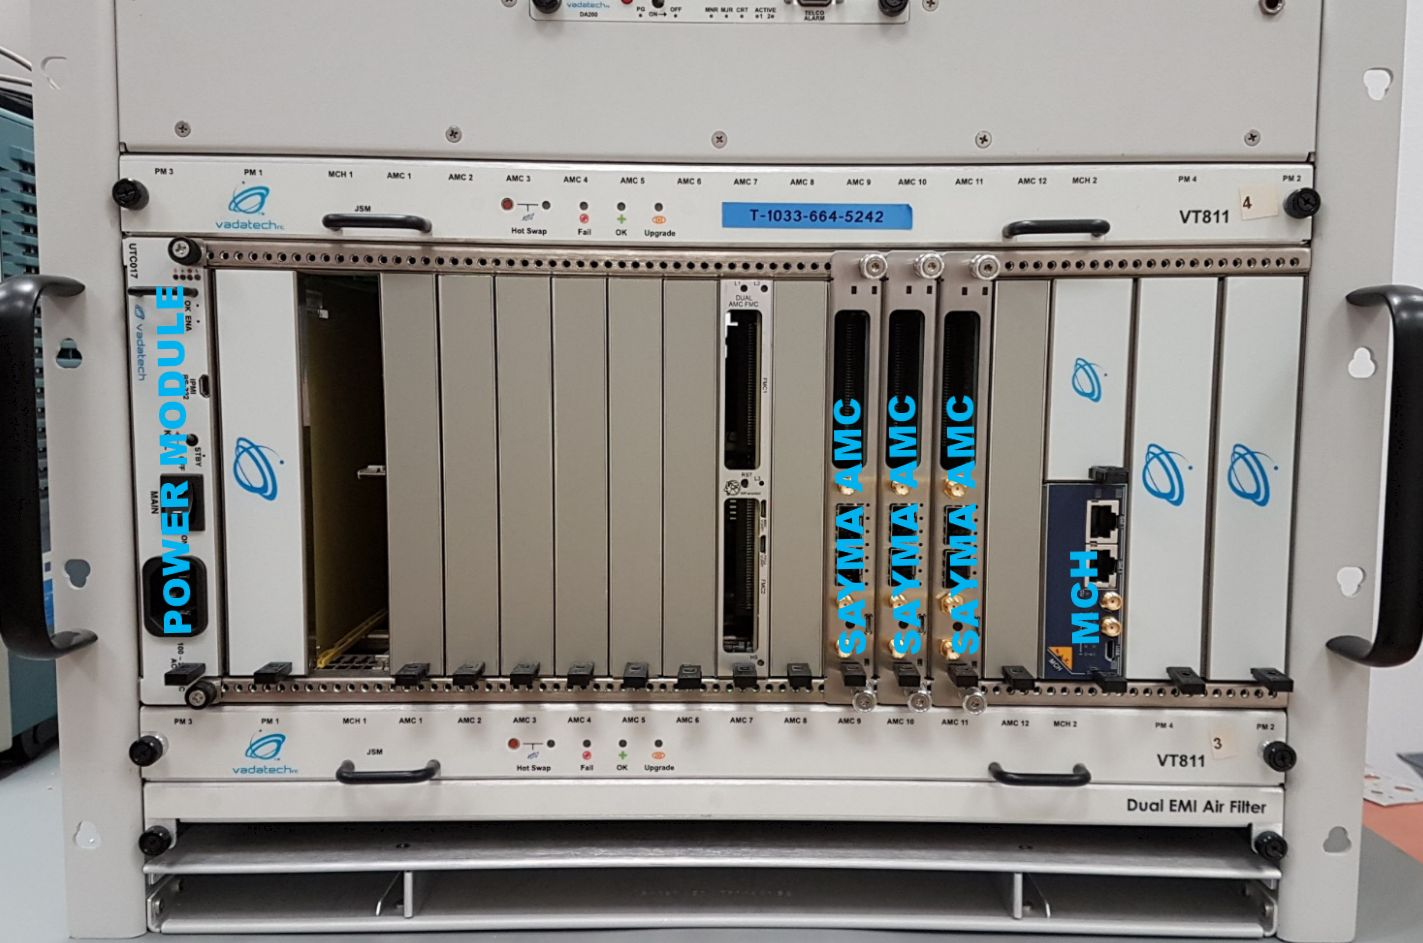
\includegraphics[width=15cm]{img/MTCA_Front1.jpg}
\caption{Micro TCA chassis with 3 Sayma AMC modules inserted}
\end{figure}

\todo[inline]{New Figure: add photo of Sayma\_AMC attached to Sayma\_RTM sitting on bench so how they're connected is clear.}

(above) Micro TCA chassis with 3 Sayma AMC modules inserted.

Micro TCA chassis with 4 RTM modules inserted. One of them with 4
BaseMod AFE mezzanines installed.

\begin{figure}[htbp!]
\centering
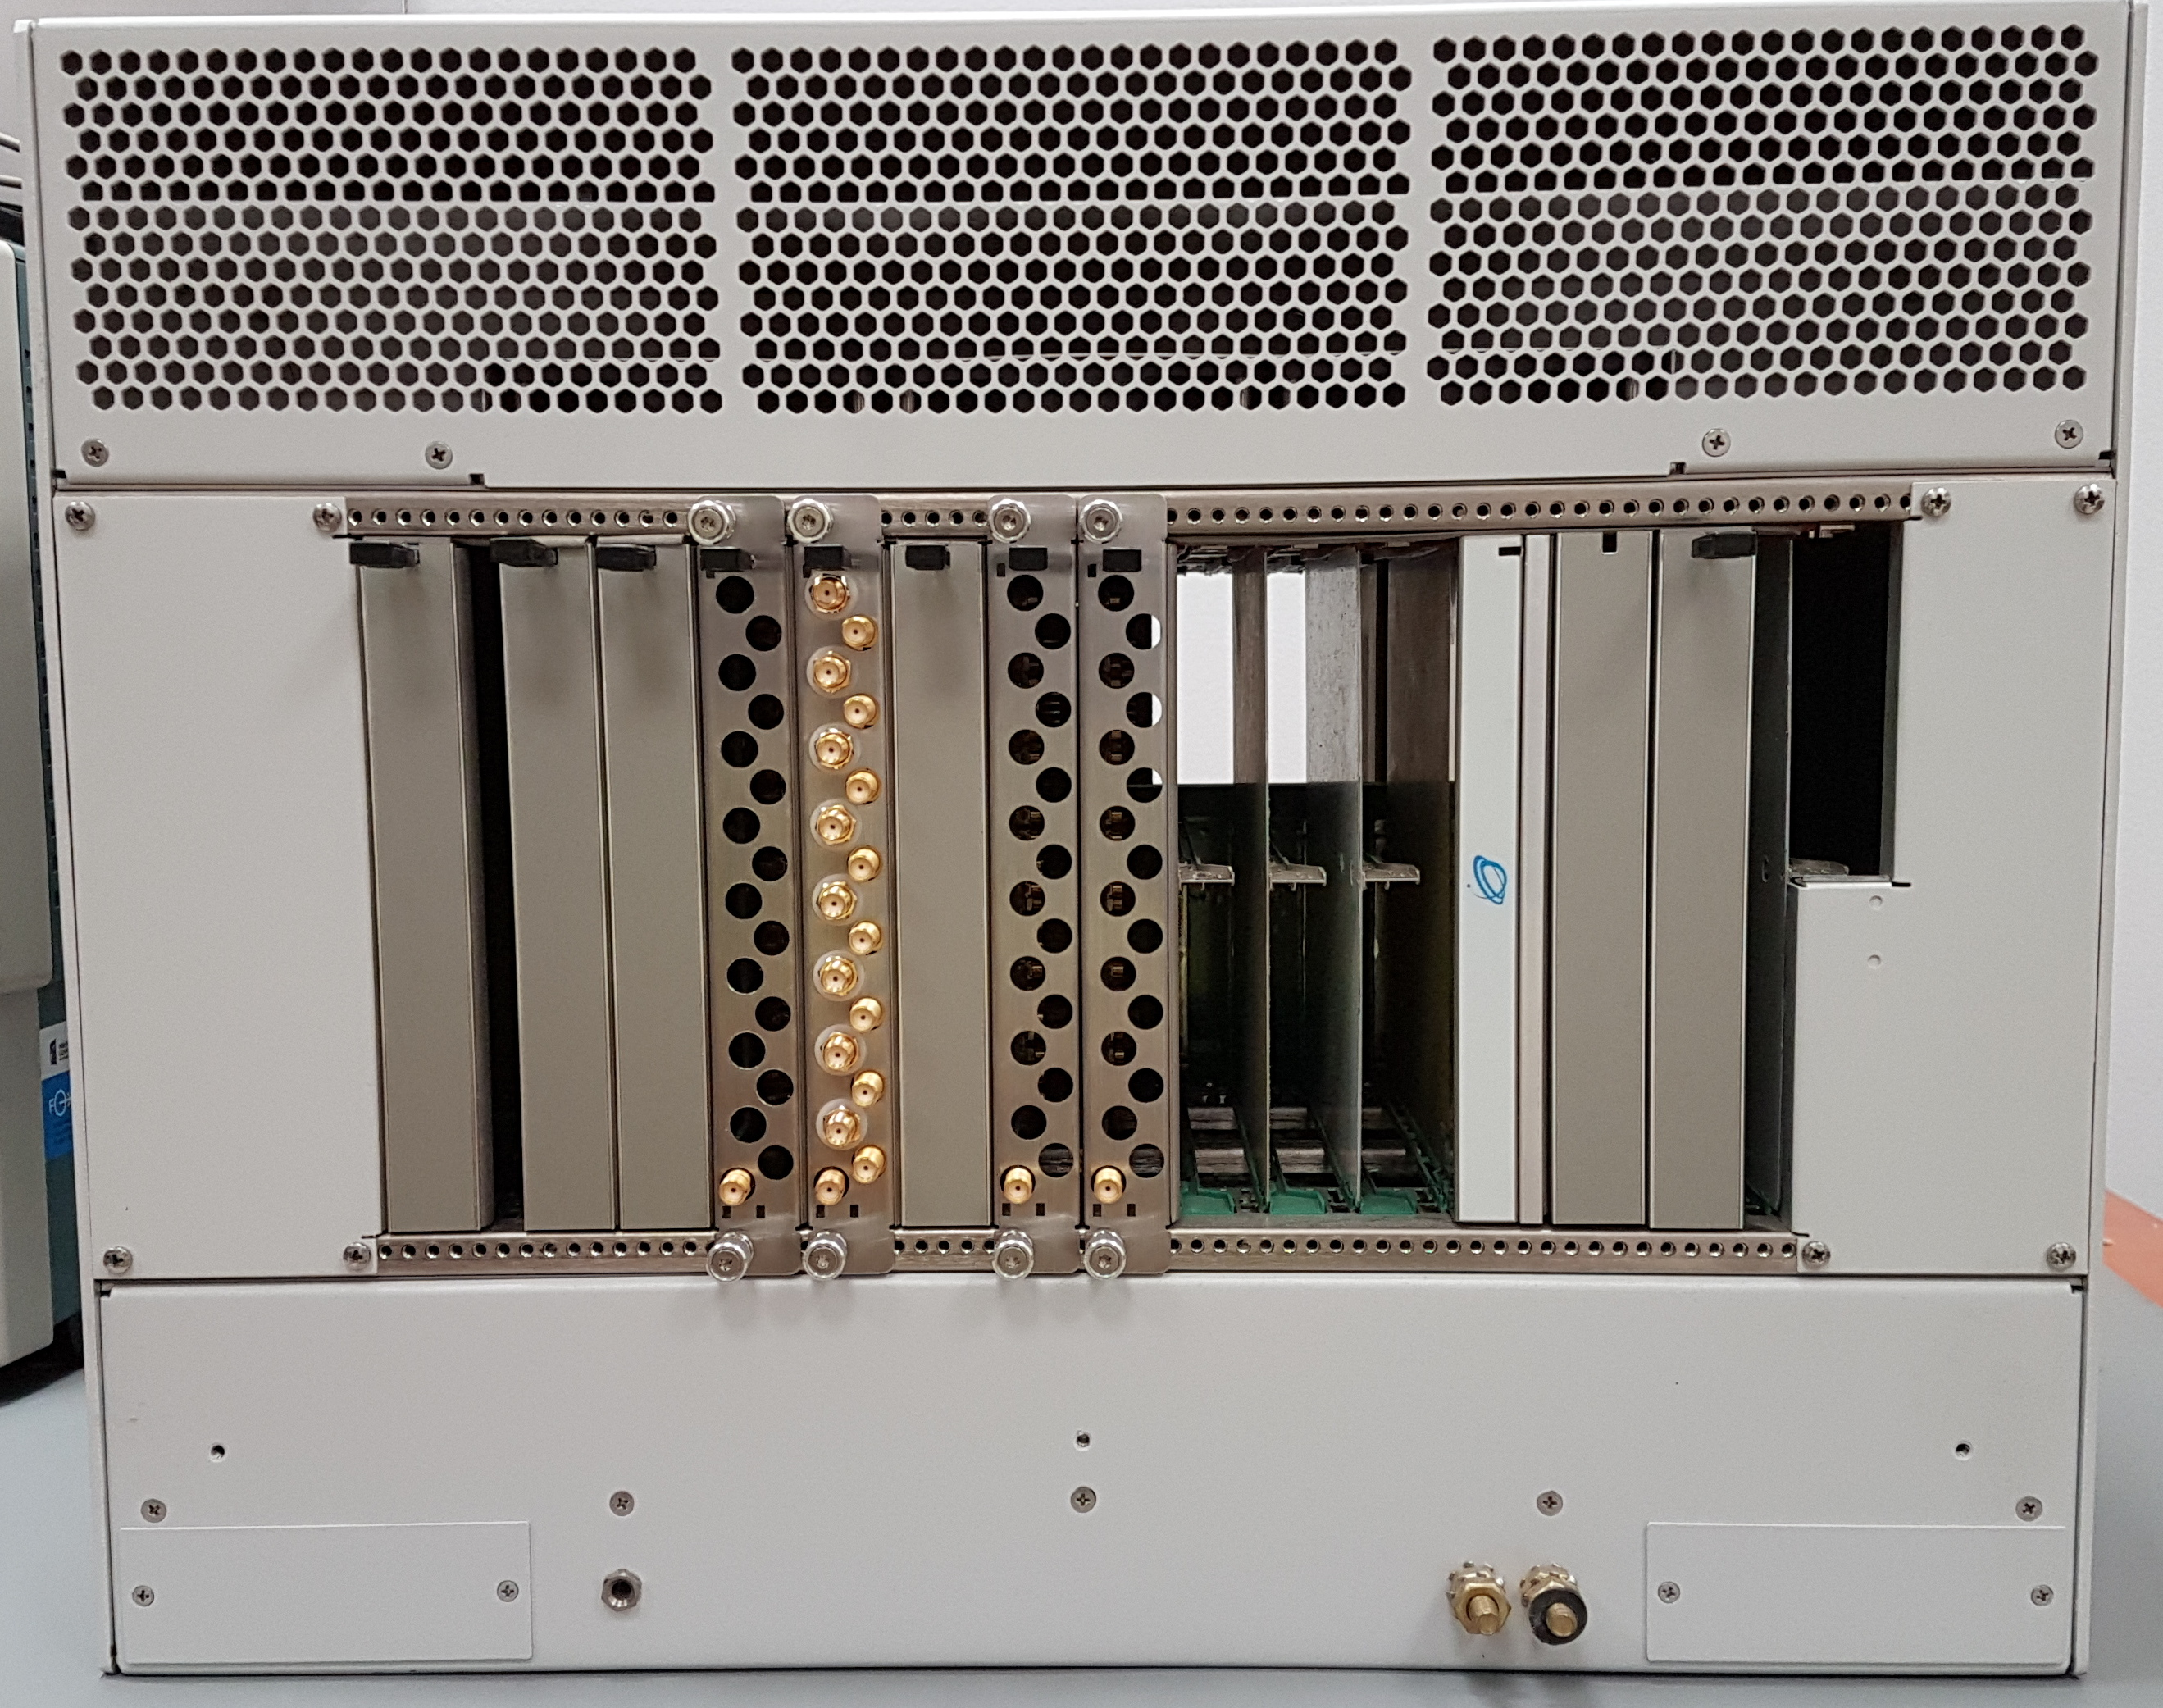
\includegraphics[width=15cm]{img/MTCA_Back.jpg}
\caption{Micro TCA chassis with 4 RTM modules inserted. One of them has
4 BaseMod AFE mezzanines installed.}
\end{figure}


\href{http://www.nateurope.com/products/NAT-LLRF-Backplane.html}{RF
BP datasheet}



\section{uTCA parts and suppliers}\label{utca-parts-and-suppliers}

\begin{itemize}
\item NAT AC 600D, qty 1
\item NAT MCH-Basic v3.5, mid-size front panel, qty 1
\item NAT Native-R5, qty 1
\end{itemize}

\section{Schematic / Layout Viewer}\label{schematic-layout-viewer}


Hardware was designed under Mentor Graphics Xpedition Enterprise and Altium Designer CAD tools.
Project resources are in two separate folders:
\begin{itemize}
	\item ARTIQ\_EE folder is for designs made with the Mentor Graphics Xpedition Enterprise CAD tool.
	\item ARTIQ\_ALTIUM folder is for designs made with Altium Designer CAD tool.
\end{itemize}
Read-only access to PCB schematics and layout designs is possible using free tools.\\
Mentor has a free tool called
\href{https://www.mentor.com/pcb/downloads/visecad-viewer/}{visECAD
Viewer}.\\
Altium has a free tool called 
\href{http://www.altium.com/altium-designer-viewer}{Altium Designer viewer}
